\section{实验尝试}
%\subsection{AdaBoost}
%AdaBoost(Adaptive Boosting, 自适应增强)是在Boosting基础上进行改进的一种集成学习算法。AdaBoost的核心思想是针对同一个训练集训练不同的分类器,即弱分类器,然后将这些弱分类器级联,得到一个强分类器。生成弱分类器时,前一个弱分类器分错的样本会得到加强,加权后的样本再被用来训练下一个弱分类器。同时将新生成的弱分类器加入到集成强分类器中,直到达到某个预定的足够小的错误率或达到预想指定的最大迭代次数。
%
%AdaBoost具体算法步骤:\footnote{\url{http://blog.csdn.net/v_july_v/article/details/40718799}}
%\begin{enumerate}
%\item 初始化训练数据的权值分布。如果有$N$个样本,则每一个训练样本最开始时都被赋予相同的权值:$\frac{1}{N}$。
%\item 训练弱分类器。具体训练过程中,如果某个样本点已经被准确地分类,那么在构造下一个训练集中,它的权值就被降低;相反,如果某个样本点没有被准确地分类,那么它的权值就得到提高。然后,权值更新过的样本集被用于训练下一个分类器,整个训练过程如此迭代地进行下去。
%\item 将各个训练得到的弱分类器组合成强分类器。各个弱分类器的训练过程结束后,加大分类误差率小的弱分类器的权重,使其在最终的分类函数中起着较大的决定作用,而降低分类误差率大的弱分类器的权重,使其在最终的分类函数中起着较小的决定作用。换言之,误差率低的弱分类器在最终分类器中占的权重较大,否则较小。
%\end{enumerate}
\subsection{AdaBoost}
AdaBoost常用的弱分类器有:CART (classification and regression tree), decision stump, SVM, logistic regress等。如果分类器过强容易产生过拟合。

\subsubsection{尝试一(MATLAB中的AdaBoost)}
20个统计特征用AdaBoost算法进行分类,实验采用的MATLAB自带函数fitensemble,最大迭代次数设为50次,实现AdaBoost算法。实验结果如图\ref{fig:19+7-matlab-adaboost-50},分类准确率为63.1\%,低于随机森林得到的分类准确率73.7\%。
\begin{figure}[!ht]
\centering
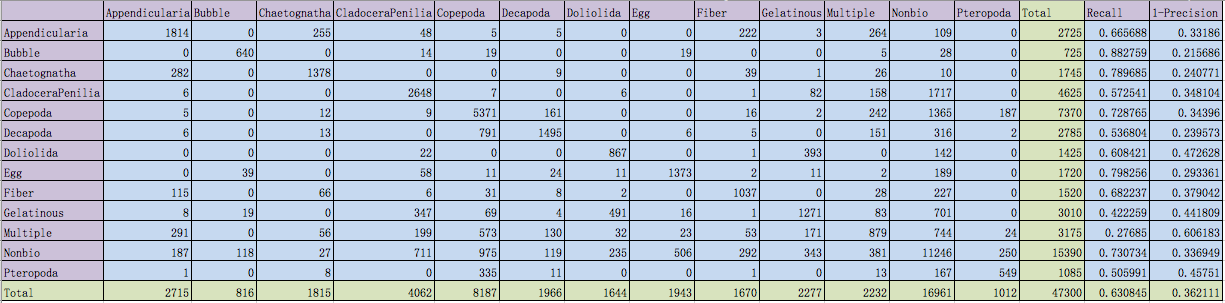
\includegraphics[width=1.0\linewidth]{19+7-matlab-adaboost-50}
\caption{20个特征采用MATLAB中的AdaBoost算法得到的分类结果}
\label{fig:19+7-matlab-adaboost-50}
\end{figure}

\subsubsection{尝试二(特征融合后采用AdaBoost)}
在特征融合方法一的基础上,将最终的分类方法SVM改为AdaBoost。实验结果如图\ref{fig:Adaboost+SVM-FeatureFusion},分类结果并没有提高。实验中遇到问题:
\begin{figure}[!ht]
\centering
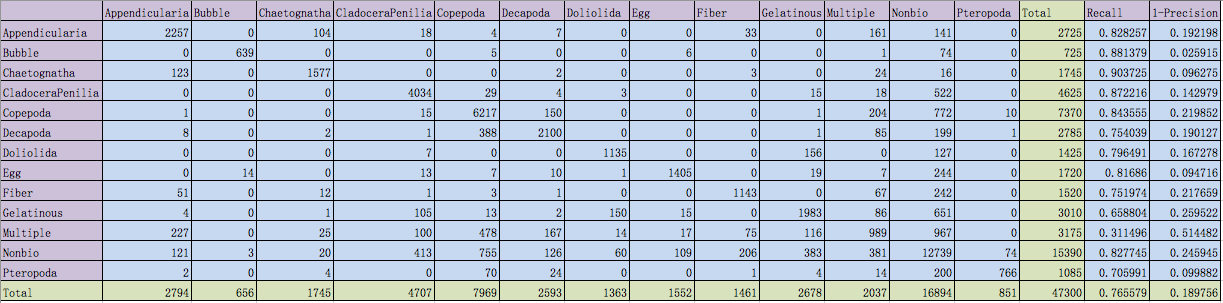
\includegraphics[width=1.0\linewidth]{Adaboost+SVM-FeatureFusion}
\caption{采用Adaboost+SVM进行特征融合}
\label{fig:Adaboost+SVM-FeatureFusion}
\end{figure}
\begin{itemize}
\item 实验中部分样本不能被识别(识别的结果13类都不是)。在实验中,我将这些不能识别的样本再用SVM进行分类。
\end{itemize}

\subsubsection{尝试三(将SVM作为弱分类器进行级联)}
该实验没有完成,在实现过程中发现两个问题:
\begin{itemize}
\item SVM作为弱分类器,在迭代的过程中不知道怎样输入样本权重。
\item 采用SVM根据已有的特征进行分类得到的分类结果已经超过50\%,这应该不是弱分类器,对它采用AdaBoost进行级联是不是会产生过拟合。
\end{itemize}

\subsubsection{AdaBoost应用}
AdaBoost可以用于:
\begin{enumerate}
\item 用于分类问题:AdaBoost应用最多的就是分类,通过级联弱分类器而得到强分类器,提高分类准确率。
\item 用于特征选择:在原始特征集合中,挑选出一些最具有代表性、可分性最好的特征子集。基于AdaBoost的特征选择过程:1、初始化训练样本权重 2、设计每个特征的分类器 3、根据加权训练样本最小错误率准则,选择分类器,也就是选择了特征 4、调整样本权重 5、通过循环,最后得到分类器的线性组合
\end{enumerate}



\subsection{Multi-view Learning}
\begin{enumerate}
\item co-training(协同训练) :是一种半指导或者无指导的学习方法,主要用于二元分类。
\item multiple kernel learning(多核学习):
\item subspace learning(子空间学习):
\end{enumerate}

\subsection{Bayes Fusion}

\subsection{Fuzzy Neural network}
模糊神经网络是模糊理论和神经网络结合的产物,是具有模糊权系数或者输入信号是模糊量的神经网络。实验结果如图\ref{fig:19+7-FNN+SVM},分类准确率为74.6\%。
\begin{figure}[!ht]
\centering
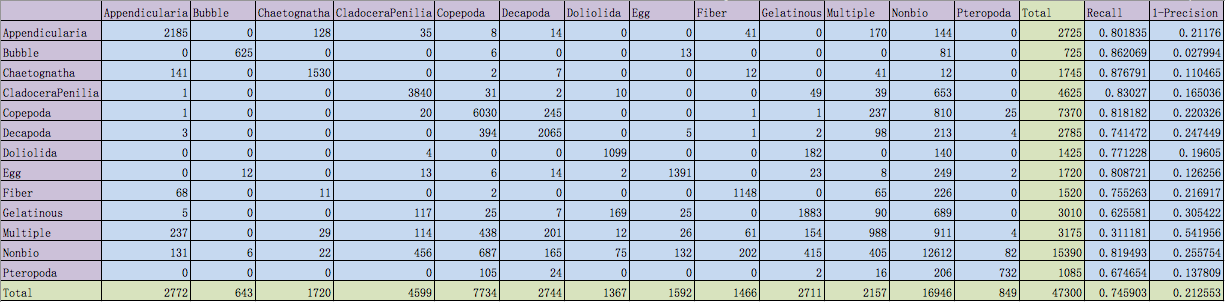
\includegraphics[width=1.0\linewidth]{19+7-FNN+SVM}
\caption{采用FNN+SVM进行特征融合}
\label{fig:19+7-FNN+SVM}
\end{figure}


%\subsection{采用AdaBoost进行浮游动物分类}
%\subsubsection{尝试一}
%想要采用20个统计特征用AdaBoost级联的SVM将浮游动物分为13类,遇到的问题:
%\begin{itemize}
%\item AdaBoost常用于二分类问题,需要进行修改。
%\item 级联SVM产生的弱分类器,没有办法设置样本的权重。
%\end{itemize}
%
%\subsubsection{尝试二}
%采用AdaBoost在特征融合方法一的基础上,将最终的分类方法SVM改为AdaBoost。由于大多的AdaBoost都是处理二分类问题,因此该实验中将分为13类转换为13个二分类问题,实验结果如图\ref{fig:Adaboost+SVM-FeatureFusion},分类结果并没有提高。实验中遇到问题:
%\begin{figure}[!ht]
%\centering
%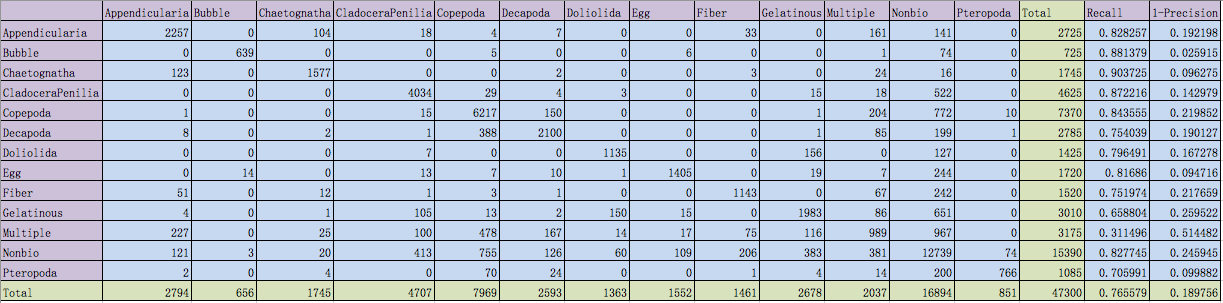
\includegraphics[width=1.0\linewidth]{Adaboost+SVM-FeatureFusion}
%\caption{采用Adaboost+SVM进行特征融合}
%\label{fig:Adaboost+SVM-FeatureFusion}
%\end{figure}
%\begin{itemize}
%\item 实验中部分样本不能被识别(识别的结果13类都不是)。在实验中,我将这些不能识别的样本再用SVM进行分类。
%\end{itemize}
%
%\subsubsection{尝试三}
%\textbf{模糊神经网络:}模糊神经网络就是模糊理论同神经网络相结合的产物,它汇集了神经网络与模糊理论的优点,集学习、联想、识别、信息处理于一体。模糊神经网络有如下三种形式:
%\begin{enumerate}
%\item 逻辑模糊神经网络
%\item 算术模糊神经网络
%\item 混合模糊神经网络
%\end{enumerate}
